\subsubsection{Hybrid Emulator}

\YIComment{Do this}

\YIComment{Do mips comparison with JIT: hybrid wins for low mips, loses for high mips}

\YIComment{Do execution time comparison with JIT: hybrid wins for low time, loses for high time}

\YIComment{Write about different hybrid variants and performance characteristics of -L and -LS: -L is great, -S is trash}

\begin{figure}[H]
    \centering
    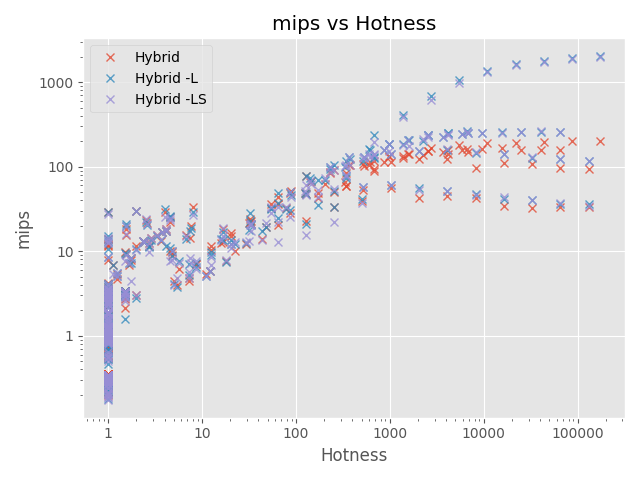
\includegraphics[scale=0.75]{output/graphs/scatter/hybrid/hotness.png}
    \caption{Performance (mips) vs hotness for all tests on the hybrid emulators.}
    \label{figure:hybrid-hotness}
\end{figure}

\autoref{figure:hybrid-hotness} shows how the performance of the hybrid emulator changes with relationship to the hotness of the programs; unlike the JIT, which has a monotonic relationship, the hybrid shows a more complex relationship.

This is because hybrid behaves like an interpreter for sufficiently cold tests, but like a JIT for sufficiently hot tests. This causes it to exhibit the `flat' performance profile of the interpreter for low hotness, before dropping in performance then rising as the JIT would. The dip in performance or the inflection point is where the hybrid begins to act like a JIT, and thus takes on all the associated overheads of a JIT, without having time make them worthwhile. This region therefore performs worse than both the interpreter or the JIT.

Naturally, we should expect the location of this inflection point to change with \texttt{-T}. Since \texttt{-T} determines how many times a block must be executed before it is compiled, it roughly corresponds to how hot a block should be before the hybrid begins emulating like a JIT; given this, we would expect the inflection to occur at higher hotness values for higher \texttt{-T}.

\YIComment{Show how that relationship changes with -T}

The ideal value for \texttt{-T} is not something that can be found through intuition; larger values will avoid more unnecessary compilation, but smaller values will cause better utilisation of the worker threads and the JIT compiler's increased execution performance.

One might logically think that the minimum value of \texttt{-T1} would lead to the highest performance on heavy test cases, but this was not found to be the case. \autoref{figure:hybrid-t-primal-mips} shows how the different values of \texttt{-T} perform on the \texttt{primal(n)} test suite.

\begin{figure}[H]
    \centering
    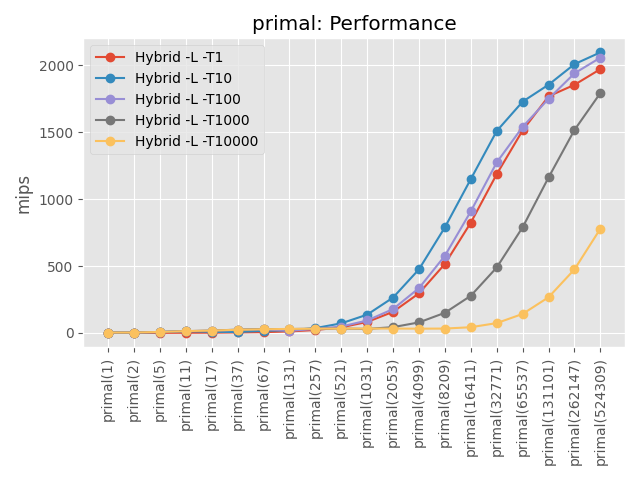
\includegraphics[scale=0.75]{output/graphs/tests/hybrid_t/primal/mips.png}
    \caption{Performance in mips of the primal test suite run on the hybrid emulator with varying values for \texttt{-T}.}
    \label{figure:hybrid-t-primal-mips}
\end{figure}

Interestingly, we observe that \texttt{-T10} has the highest performance for the intensive \texttt{primal(n)} tests; we might expect that \texttt{-T1} would hold this position as that would cause the most aggressive compilation which would eventually lead to the best performance. The most likely explanation is that \texttt{-T1} wastes too much time compiling cold blocks that are executed very infrequently and have no time to pay off (such as the entry point) causing the worker pool to be busy for longer. This would delay the compilation of the hot blocks causing the interpreter fallback to activate more frequently, despite the fact that more blocks are translated overall. We observe that larger values of \texttt{-T} cause steadily worse performance for the more intensive tests, as we might expect.

\autoref{figure:hybrid-t-primal-time} shows the execution times for the same test suite, which helps paint a far clearer picture for the performance characteristics with small \texttt{n}. We observe that \texttt{-T1} is unable to benefit from the low overhead characteristic of the emulator and begins with a relatively high execution time. Furthermore, we can that the performance at low \texttt{n} is improved as \texttt{-T} is increased. We can see that each curve behaves characteristically like the interpreter, showing a direct proportionality between the performance and \texttt{n} up until an inflection point caused by the hybrid acting more like the JIT emulator. This inflection point is similar to the one observed when investigating the relationship with hotness. Once this point is hit, the execution time becomes fairly constant before eventually curving back into a line just like with the JIT emulator. We can also see that whilst \texttt{-T10} generally performs the best, this is not universal, and it has a sour spot where it has begun compiling more blocks without having any time for it to pay off.

\begin{figure}[H]
    \centering
    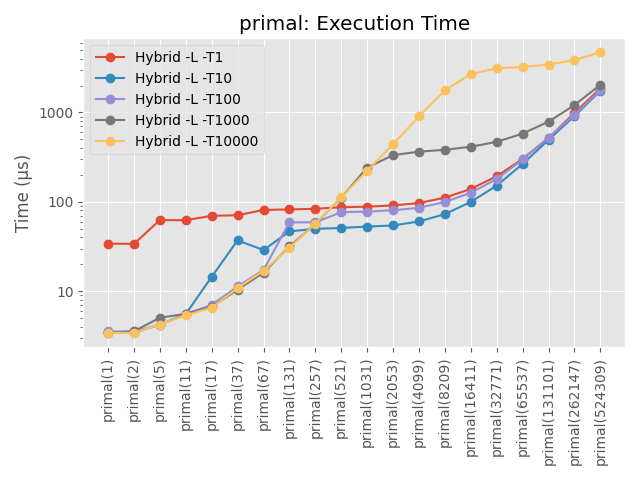
\includegraphics[scale=0.75]{output/graphs/tests/hybrid_t/primal/time.png}
    \caption{Execution time of the primal test suite run on the hybrid emulator with varying values for \texttt{-T}.}
    \label{figure:hybrid-t-primal-time}
\end{figure}

This general effect of \texttt{-T} on the performance characteristics was observed for most other test suites including \texttt{fibonacci(n)} and \texttt{memcpy(n)} as shown in \Cref{figure:hybrid-t-fibonacci-mips,figure:hybrid-t-memcpy-mips}

\begin{figure}[H]
    \centering
    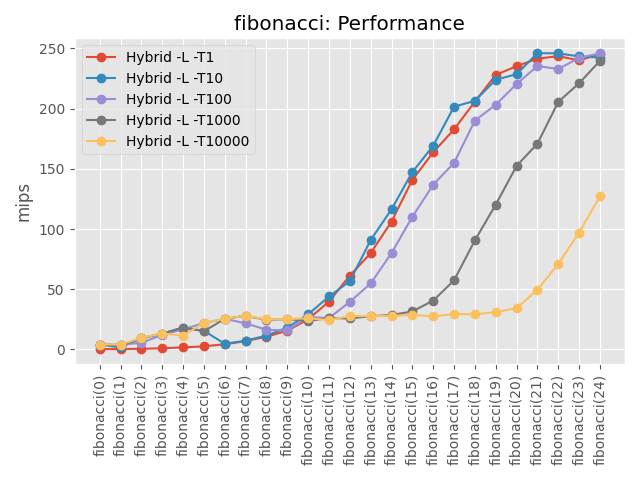
\includegraphics[scale=0.75]{output/graphs/tests/hybrid_t/fibonacci/mips.png}
    \caption{Performance in mips of the fibonacci test suite run on the hybrid emulator with varying values for \texttt{-T}.}
    \label{figure:hybrid-t-fibonacci-mips}
\end{figure}

\begin{figure}[H]
    \centering
    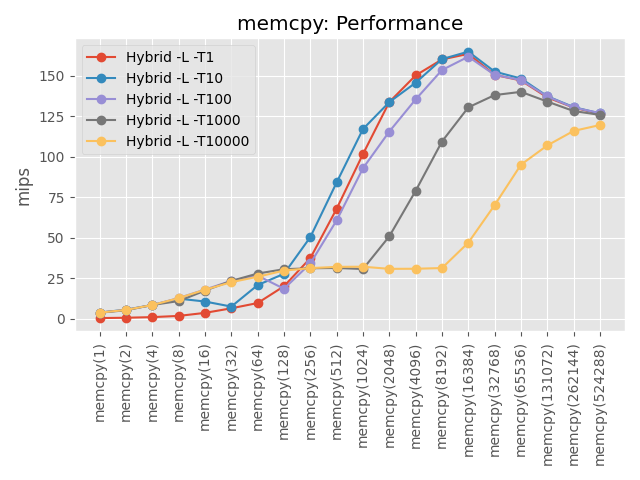
\includegraphics[scale=0.75]{output/graphs/tests/hybrid_t/memcpy/mips.png}
    \caption{Performance in mips of the memcpy test suite run on the hybrid emulator with varying values for \texttt{-T}.}
    \label{figure:hybrid-t-memcpy-mips}
\end{figure}

The ideal configuration found for the Hybrid emulator is detailed in \autoref{tbl:hybrid-optimal}

\begin{table}[H] 
    \centering
    \begin{tabular}{l|c}
        \toprule
        Option & Value \\
        \midrule
        \texttt{-L} & \cmark \\
        \texttt{-S} & \xmark \\
        \texttt{-T} & 10 \\
        \bottomrule
    \end{tabular}
    \caption{Optimal configuration found for the Hybrid emulator.}
    \label{tbl:hybrid-optimal}
\end{table}